\documentclass[tikz,border=4pt]{standalone}
\usepackage{pgfplots}\usepgfplotslibrary{groupplots}
\pgfplotsset{compat=1.18}
\definecolor{corba}{HTML}{3F51B5}\definecolor{punt}{HTML}{D32F2F}\definecolor{guia}{HTML}{6B7280}
\begin{document}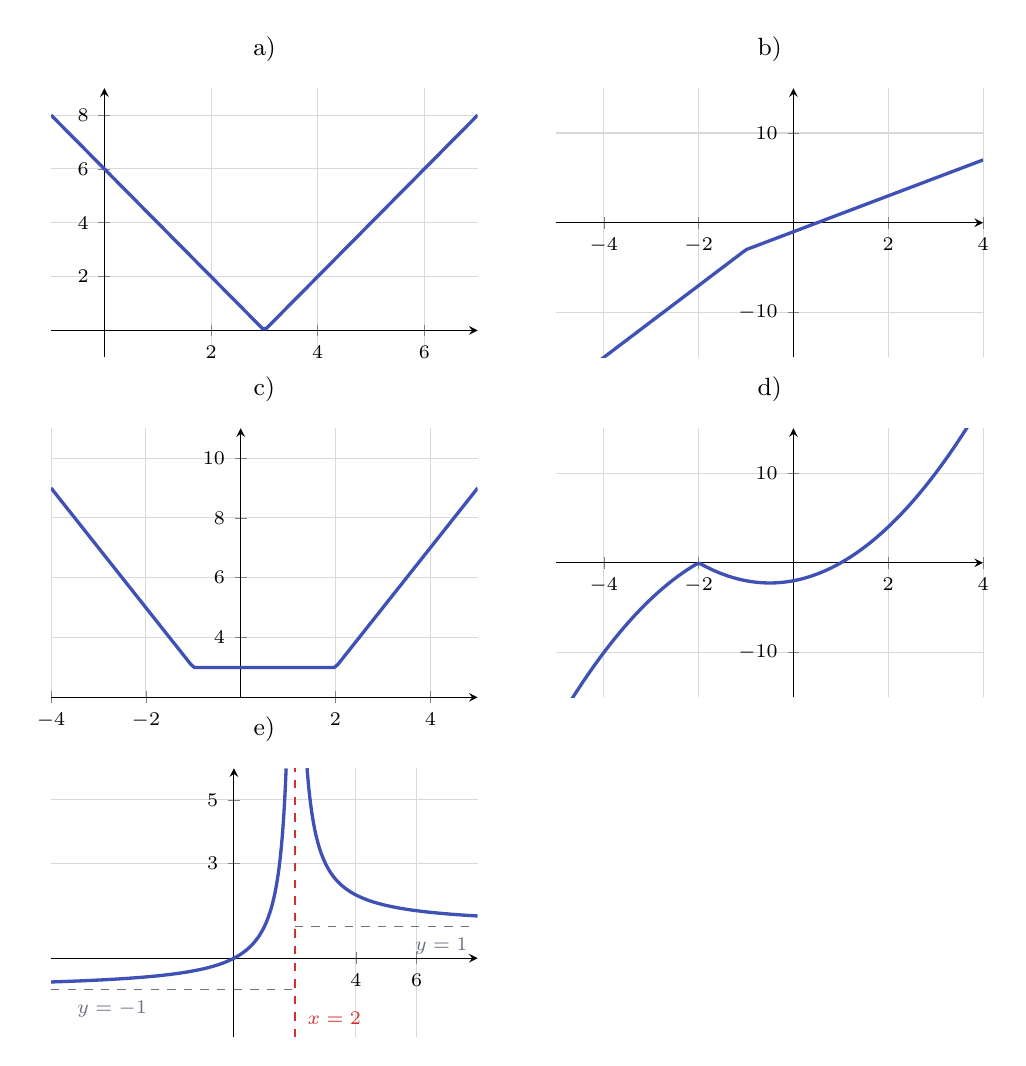
\begin{tikzpicture}
\begin{groupplot}[group style={group size=2 by 3,horizontal sep=1cm,vertical sep=0.9cm},width=7cm,height=5cm,
 axis lines=middle,grid=major,grid style={black!15},tick label style={font=\scriptsize},title style={font=\small},samples=120]
\nextgroupplot[title={a)},xmin=-1,xmax=7,ymin=-1,ymax=9]\addplot[corba,very thick,domain=-1:7]{abs(2*x-6)};
\nextgroupplot[title={b)},xmin=-5,xmax=4,ymin=-15,ymax=15]\addplot[corba,very thick,domain=-5:4]{3*x-abs(x+1)};
\nextgroupplot[title={c)},xmin=-4,xmax=5,ymin=2,ymax=11]\addplot[corba,very thick,domain=-4:5]{abs(x+1)+abs(x-2)};
\nextgroupplot[title={d)},xmin=-5,xmax=4,ymin=-15,ymax=15]\addplot[corba,very thick,domain=-5:4]{(x-1)*abs(x+2)};
\nextgroupplot[title={e)},xmin=-6,xmax=8,ymin=-2.5,ymax=6,xtick={4,6},ytick={3,5},samples=200]
\draw[punt,thick,dashed](axis cs:2,-2.5)--(axis cs:2,6);
\draw[guia,dashed](axis cs:-6,-1)--(axis cs:2,-1);
\draw[guia,dashed](axis cs:2,1)--(axis cs:8,1);
\addplot[corba,very thick,domain=-6:1.714]{x/abs(x-2)};
\addplot[corba,very thick,domain=2.4:8]{x/abs(x-2)};
\node[punt,font=\scriptsize,anchor=west] at (axis cs:2.1,-1.9){$x=2$};
\node[guia,font=\scriptsize,anchor=north] at (axis cs:-4,-1.05){$y=-1$};
\node[guia,font=\scriptsize,anchor=north] at (axis cs:6.8,0.95){$y=1$};
\end{groupplot}\end{tikzpicture}\end{document}
